\input /users/davidmcallester/icloud/tex/SlidePreamble
\input /users/davidmcallester/icloud/tex/preamble

\begin{document}

{\Huge

  \centerline{\bf TTIC 31230, Fundamentals of Deep Learning}

  
\bigskip

\centerline{David McAllester, Autumn  2024}


\vfill

\centerline{\bf Theorem Proving}

\vfill
\vfill


\slide{MathZero?}

\centerline{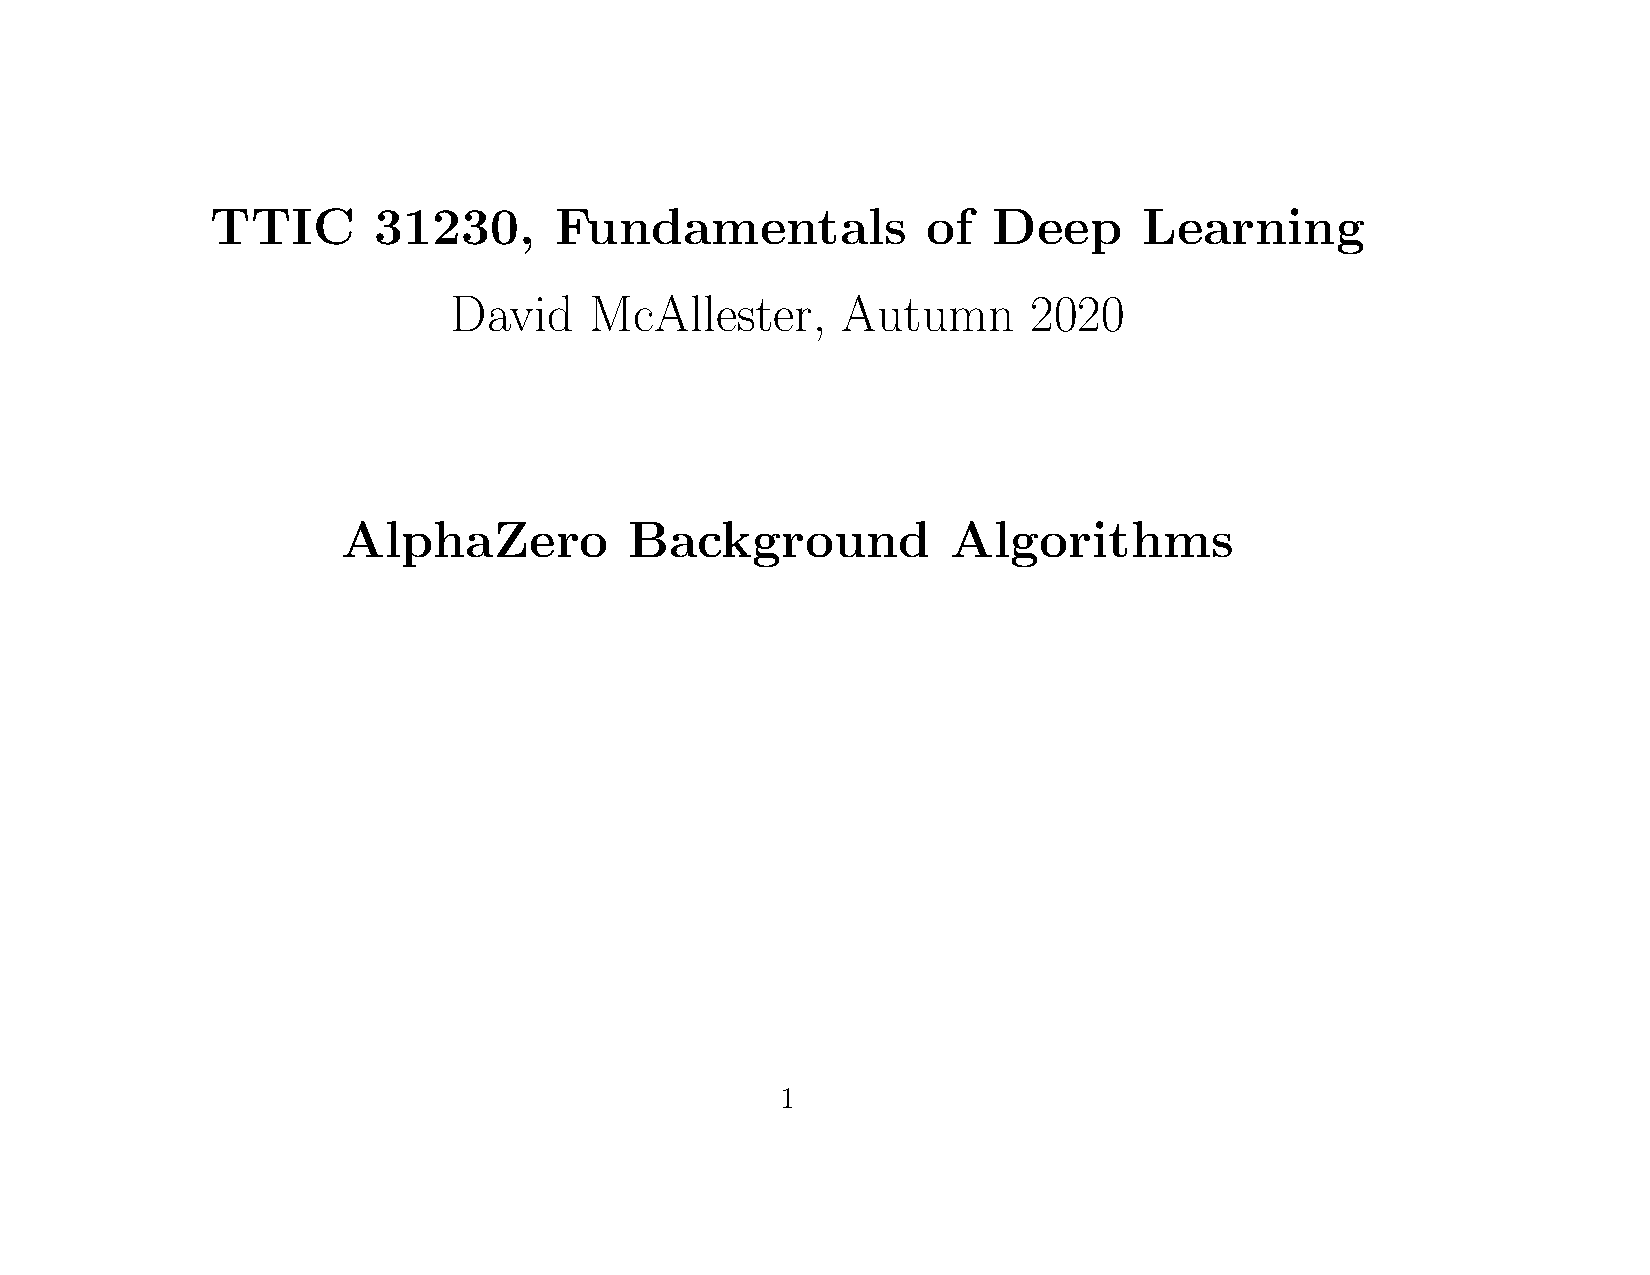
\includegraphics[height = 2.0in]{\images/alphago}}

\vfill

In 2017 AlphaZero learned to play Go, chess and shogi at a superhuman level given only the rules of the game.

\vfill
Lots of people have wondered whether something similar might be done for mathematics.


\slide{AlphaProof}

The IMO (International Math Olypiad) is an annual mathemamtics contest for high school students.

\vfill
Of the six problems in July 2024 IMO, DeepMind's AlphaGeometry solved the one geometry problem and AlphaProof solved three of the remaining five.

\vfill
The solutions were worth a silver medal.  However, AlphaProof took three days rather than the 1.5 hours humans get per problem.

\vfill
There is a blog post with a high level description (discussed below) but no paper has yet appeared.

\slide{Three Cultures}

{\bf Mathematicians (users)}: Building an AI system that can learn to play chess, Go or shogi is different from playing
chess, Go or shogi. Building a systems that can do mathematics different from doing mathematics.


\vfill
{\bf Deep Learning Researchers:} There is now a significant literature on using LLMs to generate formal proofs (LLMPGs).

\vfill
{\bf Logicians:} The developers of formal verification systems that ensure correctness 
are part of the formal methods community (programming languages, type theory, and formally sound automated reasoning).

\slide{Interest From Mathematicians}

Terence Tao (Fields Medalist) organized a group effort that machine verified one of his (coauthored) recent papers. (September 2023).

\vfill
Peter Scholze (Fields Medalist) organized a group effort that machine verified what he considered his most important theorem (2022).

\vfill
Tim Gowers (Fields Medalist) is now focusing on improving the level of automation in machine verfication systems.

\vfill
Kevin Buzzard has announced a project to machine verify Fermat's last theorem.

\slide{AlphaProof}

The blog post includes the following figure.

\centerline{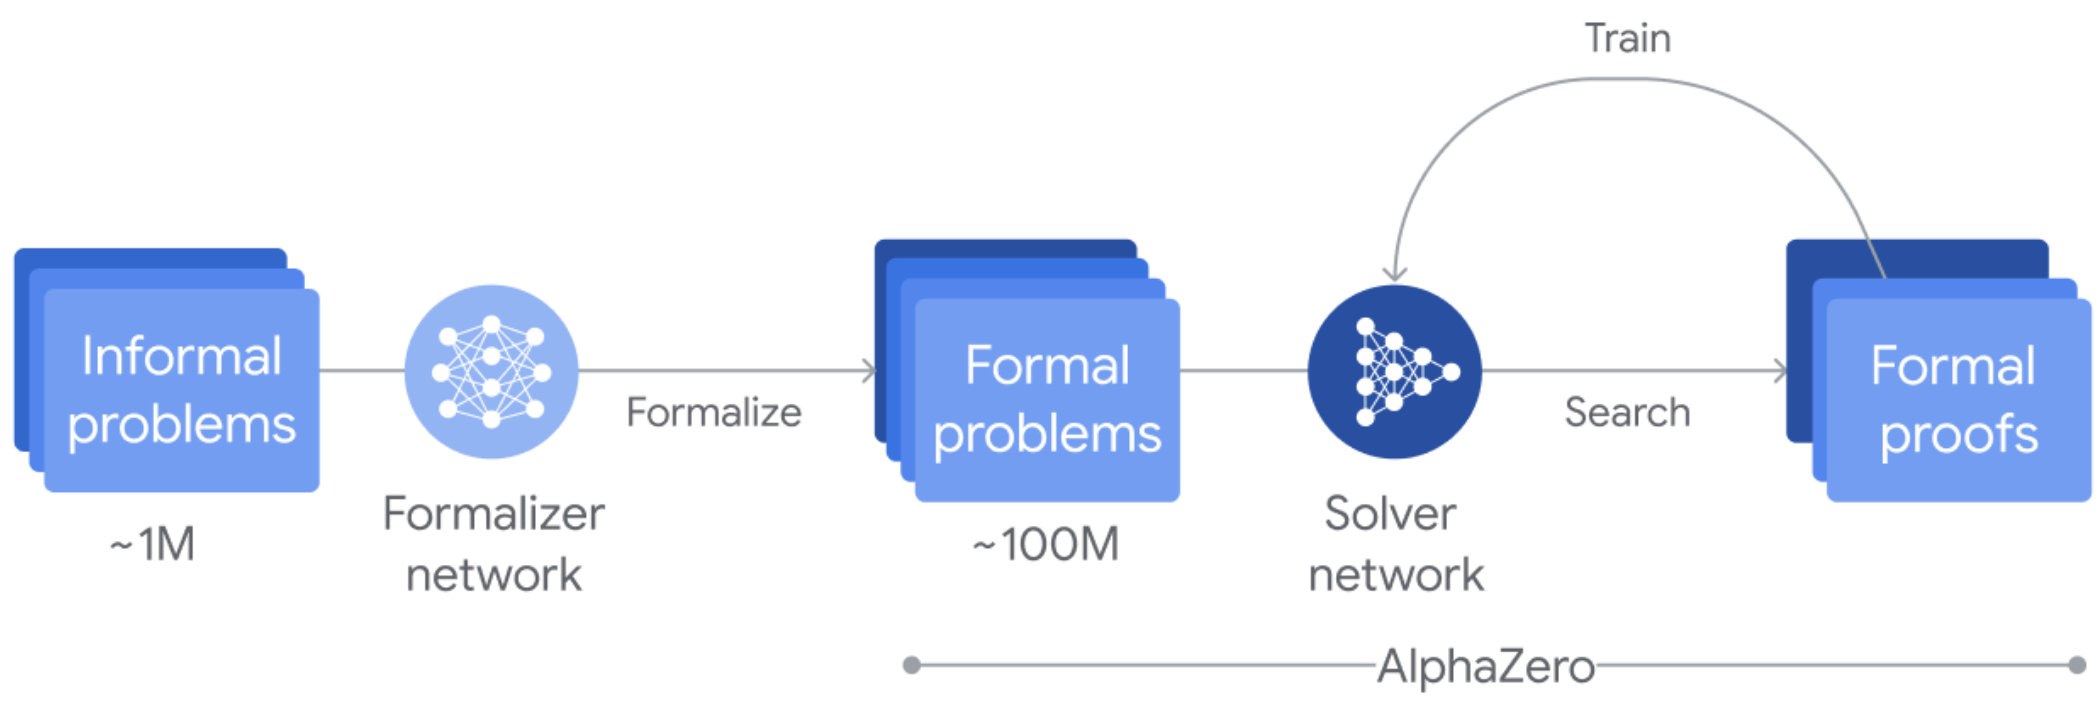
\includegraphics[width = 8in]{\images/AlphaProof}}

\slide{Research in LLMPGs}

\centerline{Generative Language Modeling for Automated Theorem Proving,}
\centerline{Polu and Sutskever, (Sept, 2020, OpenAI, cited by 223)}

\vfill
The state of the art for open source LLMPGs seems to be DeepSeek 1.5 (August 15, 2024, DeepSeek).

\slide{Logicians: The LEAN System}

By far, the dominant system for ensuring correctness is LEAN.

\vfill
{\bf Users:} Mathematician users, such as Terence Tau, Peter Scholze, and Kevin Buzzard, work directly in LEAN with possible assistance
from LLMs used in the same way that programmers use LLMs -- to make suggestions.

\vfill
{\bf Deep Learning Researchers:} Deep learning researchers are almost exclusively using LEAN to ensure correctness.

\vfill
{\bf Logicians:} I have built a system (Alfred) that is intended to be a compeitor for LEAN.

\slide{LLMPGs: Goals and Tactics}

I will call a statement that remains to be proved a goal.

\vfill
In LEAN a tactic is a function that takes a set of goals and ``backward chains'' to produce a new set of goals.

\vfill
For a proof state $S$ and tactic $T$ we have that $T(S)$ is a new set of goals such that solving $T(S)$ solves $S$.

\slide{LLMPGs: Goals and Tactics}

\vfill
For a proof state $S$ and tactic $T$ we have that $T(S)$ is a new proof state such that solving $T(S)$ solves $S$.

\vfill
For example, if a goal involves a formula such as $2x+5x$ we might use a simplification tactic to replace this expression with $7x$.
Or one might apply induction tactic on a specified well-founded order.

\vfill
For each proof state there is a choice of tactic.

\slide{AND-OR Proof Trees}

Given a set of goals we can try to solve the goals seperately by applying a tactic to each individual goal.

\vfill
This results in an and-or search tree.  At an and node we need solve all the chidren and at an or node we need to
solve only one of the children.

\vfill
HyperTree Proof Search for Neural Theorem Proving, Lample et al., May 2022 (Meta, 93 citations).

\slide{A Choice in LLMPG Architectures}

\begin{itemize}
\item {\bf AND-OR search}

\vfill
\item {\bf OR-search:} Each node is a set of goals.

\vfill
\item {\bf Whole proof generation:}
Repeatedly ask the languge model to generate
a compete proof --- a sequence of tactics that solves the given goal.

\vfill
Baldur: Whole-Proof Generation and Repair with Large Language Models, First et al, March 2023, (Google, 75 Citations).
\end{itemize}


\slide{Another Choice}

Do we insert natural language ``thoughts'' from the language model at internal nodes of the search.

\vfill
A model doing this will be called a chain-of-thought LLMPG.

\slide{More Choices}

Do we use some form of AO*-like tree growth procedure or Monte-Carlo tree search as in AlphaZero.

\vfill
Do we try to incorporate ``intrinsic'' reward into RL optimization to handle the sparse reward in mostly
failing proof attempts.

\slide{DeepSeek1.5}

DeepSeek 1.5 appears to be the state of the art LLMPG among those with a published paper.

\vfill
It uses whole proof generation but treats these as ``rollouts'' in an OR-tree.  The steps in each generated whole proof
become new nodes in the OR-tree and rollouts (whole proof generation) can be done from internal nodes.

\vfill
This is a chain-of-thought LLMPG with English thoughts at internal nodes of the tree.

\vfill
This uses monte-carlo tree search with an intrinsic reward for exploration (generating new nodes).

\slide{LLMPGs Without Formal Verification}

The blog post on alphaproof also says that they are experimenting with proofs generated entirely by natural language --- no formal verification.  They say:

\vfill

\begin{quotation}
We also tested [the language only] approach on this year’s IMO problems and the results showed great promise.
\end{quotation}

\slide{OpenAI o1 as a Proof Assistant}

Terence Tao has a Mastodon post evauating o1 as an assistant for research mathematicians. He says:

\vfill
\begin{quotation}
The experience seemed roughly on par with trying to advise a mediocre, but not completely incompetent, (static simulation of a) graduate student.
\end{quotation}

\slide{Algorithms in the Age of LLMs}

What is the role of algorithms in the age of LLMs?

\vfill
It seems unlikely that LLMs will ever replace compilers which, by deep model standards, are {\bf incredibly efficient}.

\vfill
LEAN includes certain decision procedures such as one for deciding whether an linear equation
follows from a given set of linear equations and inequalities.

\vfill
AlphaGeometry (a DeepMind geometry theorem prover) relies on Wu's algorithm from the 1970s.

\slide{Can LEAN be Strengthened?}

There are well-known algorithms for general logic that are used to great effect in SMT (Sat Modulo a Theory) software verifiers
(such as Microsoft's Z3).

\vfill
Alfred is a system that I have built based on general logic algorithms not present in LEAN.

\vfill
Alfred is intended as a competitor for LEAN.

\slide{The Schroder-Berstein Theorem}

For any two sets $s$ and $w$, if there exists an injection of $s$ into $w$ and an injection of $w$ into $s$ then there exists a bijection between $s$ and $w$.

\slide{The Schroder-Berstein Theorem}

\centerline{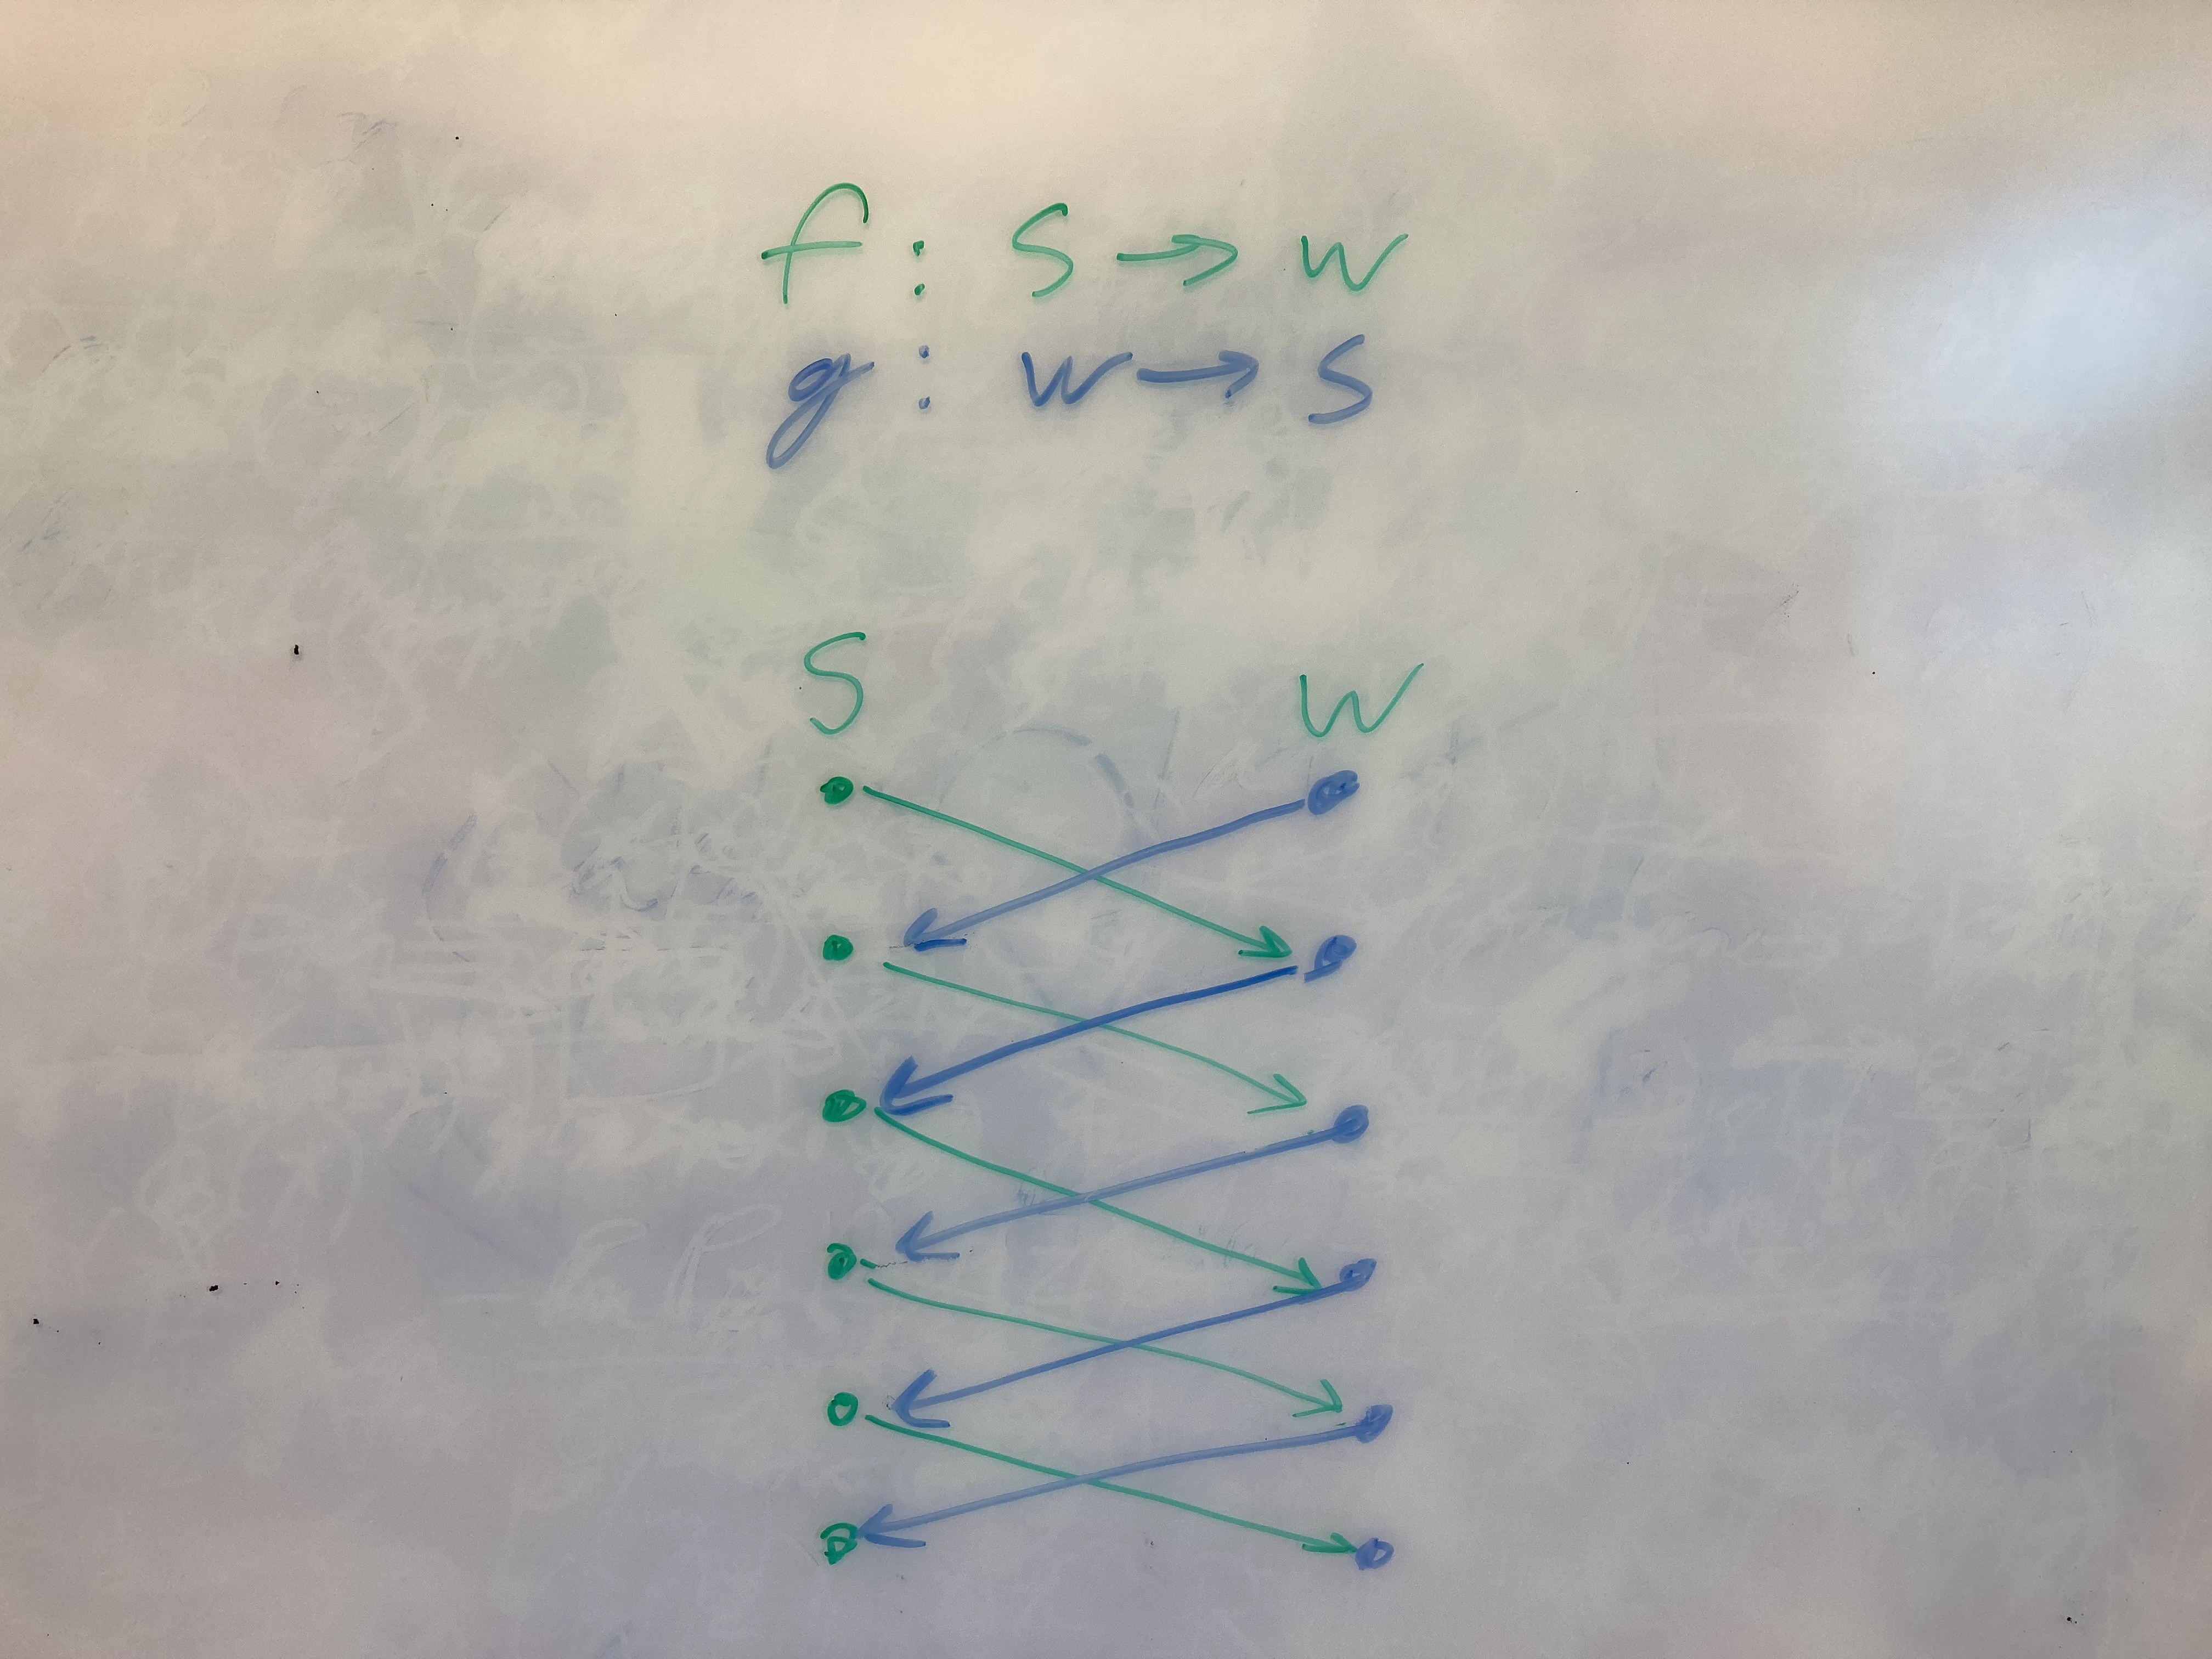
\includegraphics[width = 6.5in]{\images/SB4}}

\slide{The Schroder-Berstein Theorem}

\centerline{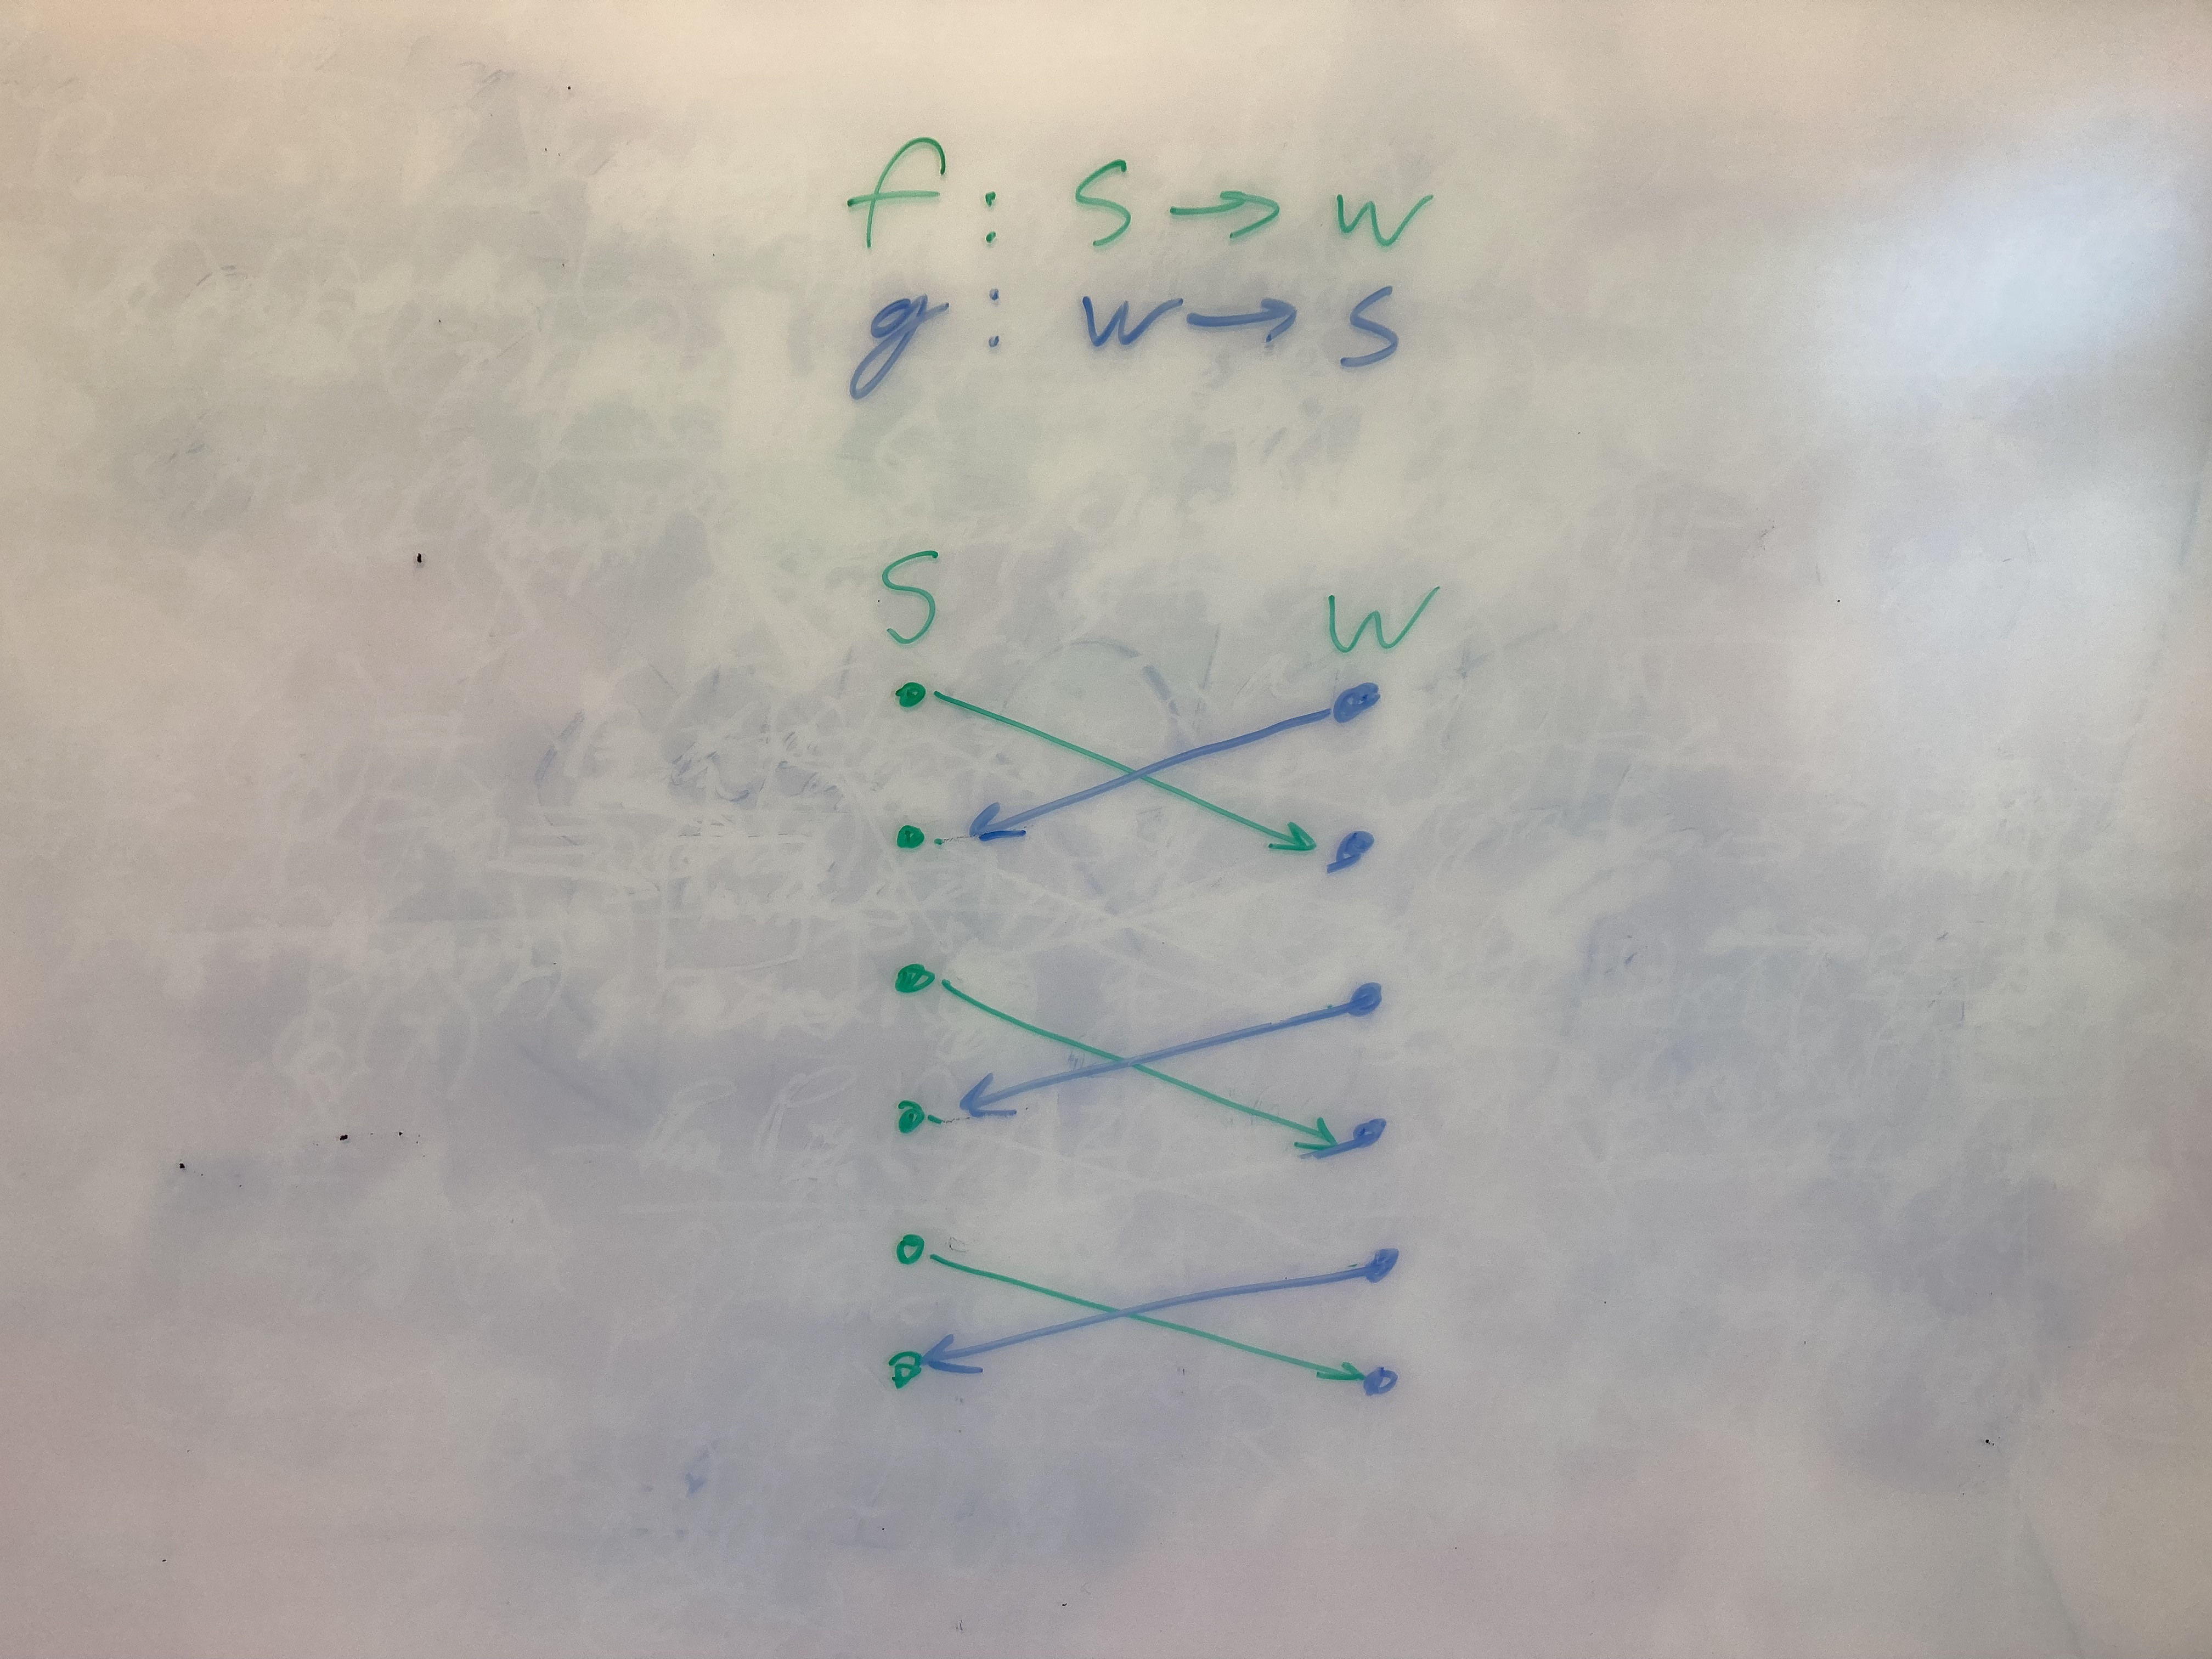
\includegraphics[width = 6.5in]{\images/SB3}}


\slide{The Schroder-Berstein Theorem in Alfred}

\centerline{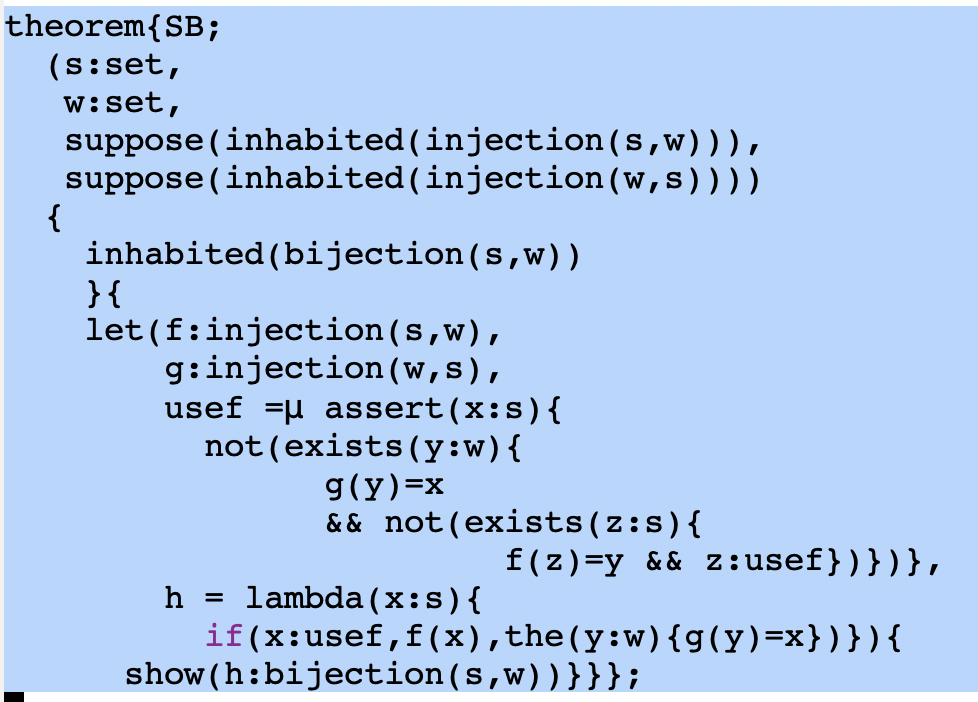
\includegraphics[width = 6.5in]{\images/AlfSchroeder}}

\slide{The Schroeder-Bernstein Theorem from LEAN's MathLib}

\centerline{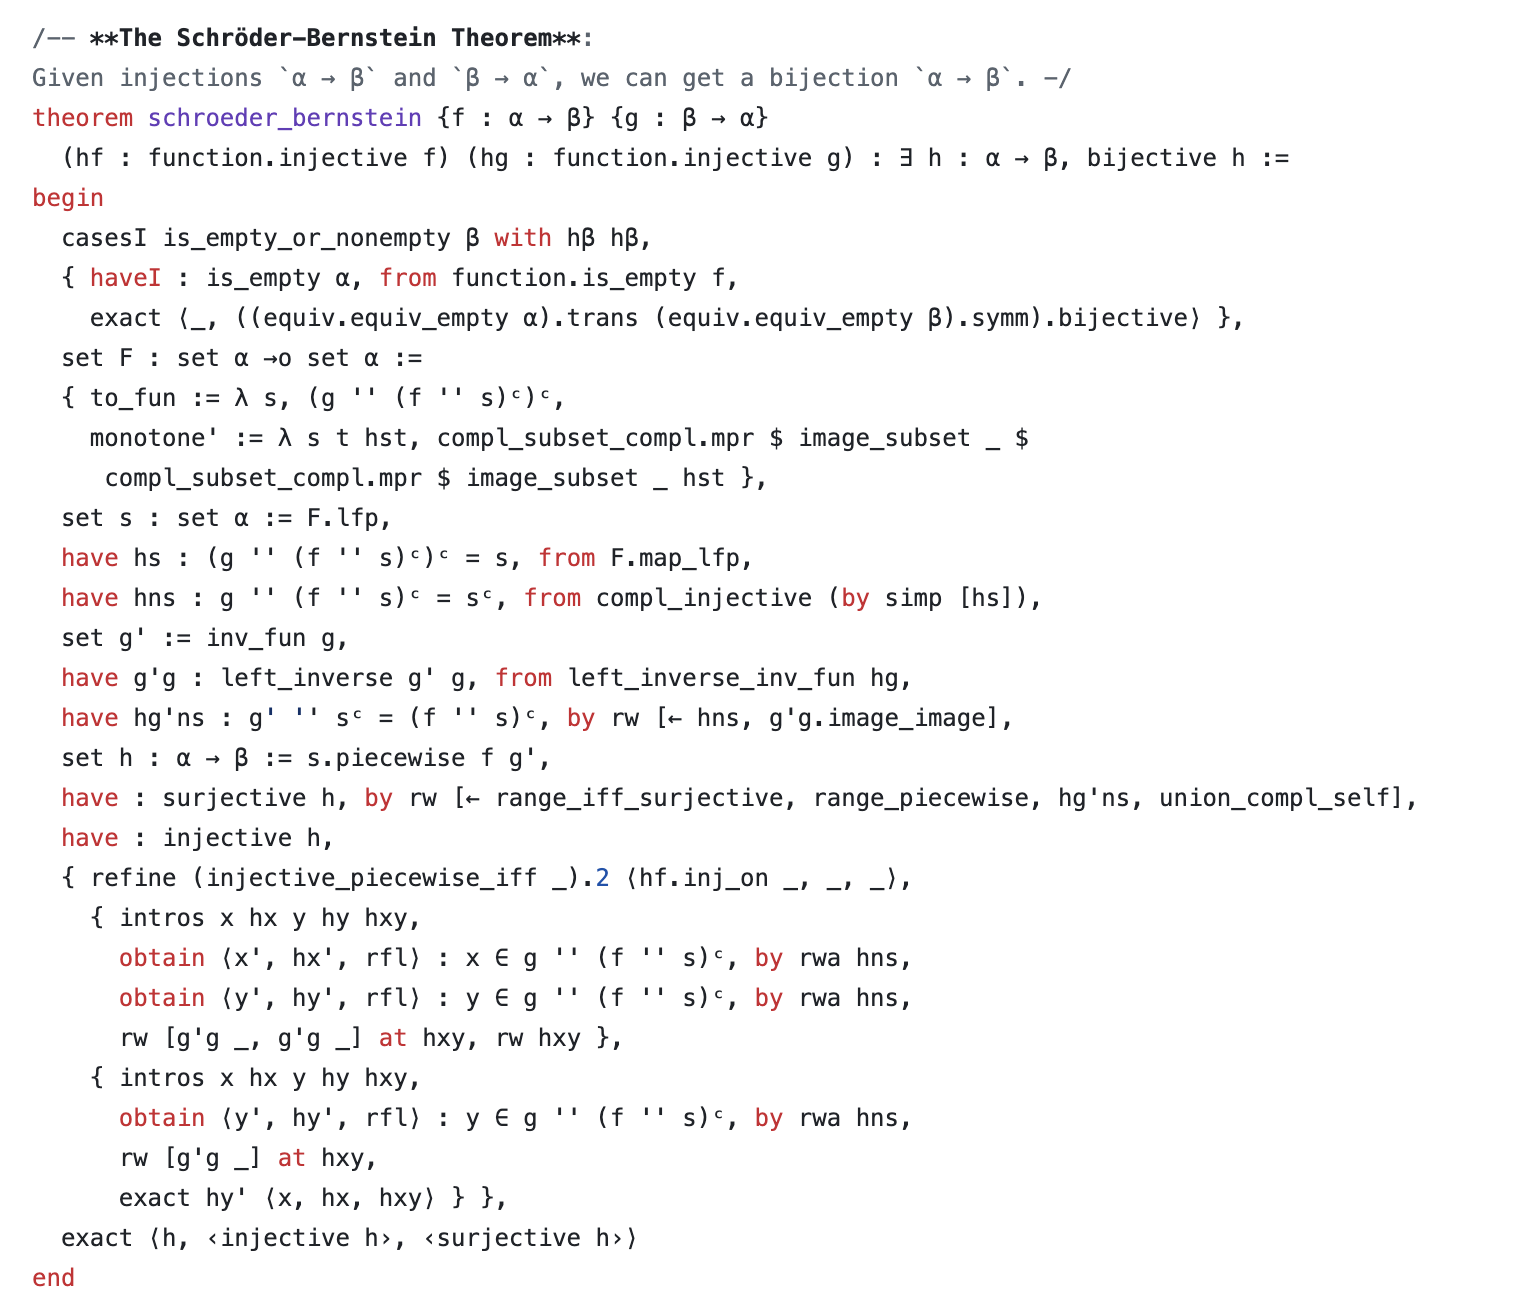
\includegraphics[width = 6.2in]{\images/Schroeder}}

\slideplain{Why Does LEAN Currently Dominate?}

{\bf Grammatical Functor Property}: Any well-typed (grammatically correct) definition of a mapping between classes denotes a {\bf functor between groupoids}.

\vfill
To explain what this means, and why it is significant, I will need to develop some background in logic.

\slide{First Order Logic}

As simple example we consider the language defined by a constant {\bf zero} and a succesor function {\bf succ}.

\vfill
In this language we can write the following axioms.

$${\color{red} \neg \exists x \;\mathrm{succ}(x) = \mathrm{zero}}$$
$${\color{red} \forall x\; (x \neq \mathrm{zero}) \Rightarrow \exists y\; x = \mathrm{succ}(y)}$$
$${\color{red}\forall x,y,z \;(\mathrm{succ}(y)= x \wedge \mathrm{succ}(z)= x) \Rightarrow y=z}$$

\vfill
But this does not pin down the natural numbers --- there are models of these axioms with
elements not reachable from zero.

\slide{The Grammar of First Order Logic}

A theorem proving system must manipulate data structures representing terms and formulas.

\vfill
The first order language  of {\bf zero} and {\bf succ} has terms and formulas
defined by the following grammar.

$${\color{red} t
::= \mathrm{variable} \;||\; \mathrm{zero} \;||\; \mathrm{succ}(t)}$$

$${\color{red} \Phi ::= t_1=t_2 \;||\; \forall x\; \Phi[x] \;||\; \exists x\; \Phi[x] \;||\; \Phi_1 \vee \Phi_2 \;||\; \Phi_1 \wedge \Phi_2 \;||\; \neg \Phi}$$


\slide{Signatures}

A first order language is defined by a set of constant, function and predicate symbols each with a specified
arity (number of arguments).

\vfill
The set of constant, function and predicate symbols together with their arity is called the {\bf signature} of the language.

\vfill
The signature defines a gammar specifying a set of {\bf grammatically well-formed} terms and formulas.

\slide{Multi-Sorted Logic}

{\huge
A multi-sorted signature consists of a set of ``sorts'' and a specification $f\!:\!\tau$ of a type $\tau$ for the each symbol $f$ of the language.

\vfill
A vector space has two sorts --- one for scalars and one for vectors.
The multiplication-by-a-scalar operator has the type specification

$${\color{red}\mathrm{SVProd}: \mathrm{scalar} \times \mathrm{vector} \rightarrow \mathrm{vector}}$$
}

\slide{Higher Order Multi-Sorted Logic}

The ``simple types'' over a given set of sorts consist of the expressions that can be constructed from the sorts, the constant type bool, and
the type constructors $\times$ and $\rightarrow$.
$${\color{red} \tau ::= \mathrm{sort} \;||\; \mathrm{bool} \;||\; \tau_1 \times \tau_2 \;||\; \tau_1 \rightarrow \tau_2}$$


\vfill
A topological space has one sort --- the points --- and an (second order) predicate {\bf open} which has the type specification
$${\color{red}\mathrm{open}:(\mathrm{point}\rightarrow\mathrm{bool})\rightarrow\mathrm{bool}}$$

\vfill
The induction axiom for arithmetic can be written as
$${\color{red}\forall P\!:\!\left(N\rightarrow\mathrm{bool})\;(P(\mathrm{zero}) \wedge \forall x\!:\!N\;P(x)\rightarrow P(s(x))\right) \rightarrow \forall x\!:\!N \;P(x)}$$

\slide{Extending Terms with Pairs and Functions}

As in programming languages, we now extend terms to include pairs, projections of pairs, functions, and applications of functions.

\vfill
Pairing {\color{red} $\tuple{s,u}$} and projections {\color{red} $\pi_1(e)$} and {\color{red} $\pi_2(e)$}.

\vfill
$\lambda$-expressions (functions) {\color{red} $\lambda\; \intype{x}{\tau}\;e[x]$} and applications {\color{red} $f(e)$}.

\vfill
It is not difficult to define the grammar of this extended set of terms.

\slide{Signature-Axiom Classes}

Common mathematical concepts can be defined as models of a multi-sorted signature satifying given axioms written in the language defined
by the signature.

\vfill
Intuitively we have a ``data type'' specified by the signature.  An instance of this data type is a model
(particular data) specifying a value for each sort
and a value for each declared symbol (consistent with the type declarations).

\vfill
We also have ``axioms'' which are the properties that the data must satisfy.  We assume the axioms to be grammaticaly well-formed (well typed).

\slide{The Signature-Axiom Groupoid}

Two structures of the same signature are isomorphic if there exists a system of bijections between the sorts which carry the data of one to the data of the other.

\vfill
It is straightforward to define the notion of ``carry'' for simply typed language constants.


\vfill
It is also straightforward to prove that
if two models of the same signature are isomorphic then they satisfy the same (grammatical) formulas.

\vfill
We then get that every signature-axiom class defines a groupoid --- a category in which every morphism is an isomorphism.

\slidetwo{We now have Groupoid Classes.}{What About Functors?}

We want a formal language for expressing functions (functors) between groupoids.

\vfill
We want that isomorphic graphs have the same graph Laplacian because the definition of the graph Laplacian is grammatically well-formed (well typed).

\vfill
We want that isomorphic topological manifolds have isomorphic homotopy groups because the definition of the homotopy group is grammatically well-formed (well typed).

\slide{LEAN's Advantage}

{\bf Grammatical Functor Property}: Any well-typed (grammatically correct) definition of a mapping between classes denotes a {\bf functor between groupoids}.

\vfill
This implies that one can substitute isomorphic objects into any {\bf well typed} context.

\vfill

~ \hfill\unnamed
    {
      \ant{\Gamma \models f:\sigma \rightarrow \tau}
      \ant{\Gamma \models u =_\sigma v}
    }{
      \ant{\Gamma \models f(u) =_\tau f(\sigma)}
      }
\hfill ~

\vfill

\slidetwo{The Importance of Isomorphism:}{Classification}

Classification is a central objective of mathematics.  Classifying the finite groups, or topological manifolds, or differentiable manifolds, or Lie groups.

\vfill
Classification is ``up to isomorphism''.

\vfill
We can expect an autonomous AI mathematician to naturally be oriented toward classification problems.

\slidetwo{The Importance of Isomorphism:}{Representation}

Any two three-dimensional vector spaces over the reals are isomorphic (although there is no natural or canonical isomorphism).

\vfill
$\mathbb{R}^3$, defined as the set of triples of real numbers, is a representation of a three dimentional vector space over the reals.

\vfill
``Representation theory'' is the study of the representation of groups as linear operators on vector spaces.

\slidetwo{The Importance of Isomorphism:}{Cryptomorphism}

People immediately recognize when two different types are ``the same'' or ``provide the same data''.

\vfill
A group can be defined in terms of the group operation, the identity element, and the inverse operation, or alternatively, just
the group operation.

\vfill
Birkhoff (1967) called the relationship between these two fomulations of group a cryptomorphism.

\vfill
Two classes $\sigma$ and $\tau$ are cryptomorphic if there exists well-formed functors $\intype{F}{\sigma \rightarrow \tau}$
and $\intype{G}{\tau \rightarrow \sigma}$ whose composition is the identity.

\slidetwo{The Importance of Isomorphism:}{Symmetry}

Any $x$ of type $\tau$ has a $\tau$ symmetry group --- the set of $\tau$-automorphisms of $x$ (isomorphisms of $x$ with itself).  For example a geometric
circle has rotational and reflective symmetries.

\vfill
If $x\!:\!\tau$ and $y\!:\!\sigma$ are $\tau$-$\sigma$-cryptomorphic then the $\tau$ symmetry group of $x$ must be isomorphic (as a permutation group) to the $\sigma$ symmetry group of $y$.

\vfill
If we treat cryptomorphic objects as just different expressions of ``the same data'' then an object has no natural or canonical structure beyond its symmetry group.


\slide{The Role of Constructivism}

The grammatical functor property was proved for Martin-L\"{o}f type theory, from which LEAN is derived, by Hofmann and Streicher in 1995.

\vfill
But Martin-L\"{o}f type theory (1972) was motivated entirely by constructivism.


\vfill
It turns out that there is no need for constructivism.  The success of LEAN should not be viewed as a vindication of constructivism.

\vfill
This talk presents a dependent type system satisfying the grammatical functor property but derived as a direct generalization of the semantics of multi-sorted higher-order logic.

\slidetwo{Constructive Logic:}{Propositions as Types}

Constructive logics formulate propositions as the types of computer programs.

\vfill
Proof checking is reduced to type checking.

\vfill
A proof of $P$ is a well-typed program whose type is $P$.

\vfill
Constructive logic must be extended with the excluded middle and the axiom of choice to support working mathematicians.

\slide{Semantics}

Constructive logic is specified by inference rules.

\vfill
Following Tarski (1933) we have specified logics {\bf semantically}.

\vfill
We write $\Sigma \models \Phi$ to mean that $\Phi$ is true in all models of $\Sigma$.

\vfill Semantics defines soundness and completeness and is needed to formulate G\"{o}del's incompleteness theoerms.

\vfill
We will continue to work semantically and simply generalize a little further the logic developed so far.

\slide{First Class Sorts}

In a programming language something is ``first class'' if it can be passed as an argument to a procedure and included as a value in data structues.

\vfill
A group contains its sort as part of its data (the set of group elements).

\vfill
To define the type ``group'' we need sorts to be included in objects --- we need first class sorts.

\slide{ Dependent Pair Types}

\vfill
To support first class sorts we now include {\color{red} $\mathrm{set}$} as a type so that we can declare a sort $s$ with
{\color{red}$s:\mathrm{set}$}.

\vfill
We generalize {\color{red} $\sigma \times \tau$} to {\color{red} $\Sigma_{\intype{x\;}{\;\sigma}}\;\tau[x]$} which denotes the set of all pairs $\tuple{x,y}$ with $x \in \sigma$ and $y \in \tau[x]$.

$${\color{red} \mathrm{magma}: \Sigma_{s:\mathrm{set}} [s\times s \rightarrow s]}$$

\slide{Dependent Function Types}

We generalize {\color{red} $\sigma \rightarrow \tau$} to {\color{red} $\Pi_{\intype{x\;}{\;\sigma}}\;\tau[x]$} which denotes the set of all functions $f$ such that the domain of
$f$ is $\sigma$ and for all $x \in \sigma$ we have $f(x) \in \tau[x]$.

\vfill
$${\color{red} \mathrm{\mathrm{cons}}: \Pi_{\alpha:\mathrm{set}}\; (\alpha \times \mathrm{listof}(\alpha)) \rightarrow \mathrm{listof}(\alpha)}$$

\slide{Axioms}

Axioms can be incoporated into the type system with ``some such that'' types technically known as {\bf restriction types}.

\vfill
The some-such-that type {\color{red}$S_{x:\tau}\;\Phi[x]$} denotes the type of those values $x:\tau$ satisfying the ``axiom'' $\Phi[x]$.

\vfill
$${\color{red} \mathbf{Group} \; \equiv \; \Sigma_{\intype{s\;}{\;\mathrm{Set}}}\;S_{\intype{f\;}{\; s\times s \rightarrow s}}\;\Phi[s,f]}$$
\vfill

\slide{Constructive Logic ``Axioms''}

It seems natural to represent a group as a signature-axiom class.

$$\mathbf{Group} \; \equiv \; \Sigma_{\intype{s\;}{\;\mathrm{Set}}}\;{\color{red} S}_{\intype{f\;}{\; s\times s \rightarrow s}}\;\Phi[s,f]$$

\vfill
In constructive type theories one replaces the restriction type
with a pair type.

$$\mathbf{Group} \; \equiv \; \Sigma_{\intype{s\;}{\;\mathrm{Set}}}\;{\color{red} \Sigma}_{\intype{f\;}{\; s\times s \rightarrow s}}\;\Phi[s,f]$$

\vfill
Here a proof of the axioms must always be given as part of the data of the group.


\slide{The Signature-Axiom Distinction in Programming}

\vfill
In a typed programming language a procedure is declared by specifying types for its arguments and return value.  This declaration is called the ``signature'' of the procedure.

\vfill
Programming languages also support ``assertions'' --- run-time checks on program invariants.  For example, one might assert that at this point
in the program the variable $x$ is an even number.

\vfill
Compile-time checking of assertions is undecidable. Assertions become run-time checks.


\slide{Alfred}

Alfred, named for Alfred Tarski, is an under-development system intended to compete with LEAN.

\vfill
Any competitive advantage over LEAN will be due to the level of automation.  Time will tell ...


\slide{The Signature-Axiom Distinction in Alfred}

Alfred has a decidable {\bf signature-checking} algorithm for the type system defined here analogous
to type checking in programming language with run-time assertions.

\vfill
For a mathematical verification system we also want {\bf axiom-checking}. If $f$ is a functor taking a group as an argument
we want to check that in any application $f(G)$ we have that $G$ is a group.

\vfill
This is analogous to verifying the run-time assertions in a computer program.

\slide{Handling Undecidability}

Alfred has a quickly terminating but incomplete axiom-checker.  We make this as strong as possible while preserving quick termination.

\vfill
If the axiom-checker fails to prove that $G$ is a group we can first provide an explicit proof.

\slide{Variants of Dependent Type Theory}

\vfill
I will reserve the term ``dependent type theory'' for type system satisfying the grammatical functor property.

\vfill
In practice such a system should be given a ZFC-complete inference mechanism (rules or algorithms).

\vfill
Just as with typed programming languages, among dependent type theories the choice of particular language features matters.

\vfill
Of particular interest is object-oriented type systems.


\slidetwo{Speculation:}{The Grammar of Mathematical Natural Language}

Just as in all human languages, human mathematical language has grammar.

\vfill
Dependent type theory can be interpreted as a formal treatment of the grammar of the natural language of mathematics.

\slidetwo{Speculation:}{Object-Oriented Everything}
Modern programming languages support object-oriented programming.

\vfill
Mathematics is object-oriented in the sense that one deals with classes, such as the class of groups, and instances.

\vfill
Class-instance structure (object orientation) underlies natural language semantics (Fillmore 1976).

\vfill
Perhaps large language models will eventually make a transition from the transformer to an object-oriented archiecture.


\slidetwo{Speculation:}{What is an Electron?}

If we view cryptomorphic objects as ``the same data'', and we view objects with the same symmetry group as cryptomorphic,
then a mathematical object has no natural or canonical structure beyond its symmetry group.
It then seems natural that an electron (or the value space of the electron field) has no identifiable structure
beyond its symmetry group.



\slide{Summary: The Grammatical Functor Property}

\vspace{-.5in}
~ \hfill\unnamed
    {
      \ant{\Gamma \models f:\sigma \rightarrow \tau}
      \ant{\Gamma \models u =_\sigma v}
    }{
      \ant{\Gamma \models f(u) =_\tau f(\sigma)}
      }
\hfill ~

\slide{END}

}
\end{document}


\slide{Some History: Bourbaki}

Bourbaki (1939) defined ``structure'' and isomorphism.

\vfill
However, the notion of structure is not as general as that of dependent type theory and,
more significantly, Bourbaki did not define the grammatically correct class of expressions for which substitution holds.

\slide{Some History: Type Theory}

Type theory appeared in Russel and Whitehead's Principia Mathematica (1910).

\vfill
Dependent type theory grew out of Brouwer's (1914) program of constructive mathematics.
Constructive mathematics has been largely ignored by mathematicians
but survives in the study of types for programming languages.

\vfill
Dependent type theory reached its modern form in Marten-L\"{o}f type theory (1972),
and Coq (1989), the ancestor of LEAN (2010).

\vfill
The substitution of isomorphics was formulated in the groupoid model of Martin-L\"{o}f type theory (Hofmann and Streicher, 1995).

\slide{Misguided (IMHO) Trends in Type Theory}

Constructivism: Constructivism is largely ignored by practicing mathemticians. Dependent type theory is more natural without it.

\vfill
The restriction in Coq and LEAN that every object has a unique type contradicts mathematical practice and should
be dropped --- an Abelian group is a group and a Lie group is a group.


\vfill
Homotopy type theory is not taken seriously and should be dropped.  Isomorphism is based on bijections not
homotopy paths.

\slide{END}

\end{document}


